This section elaborates on our results starting from an overview of a randomly-selected, statistically-relevant subset (i.e., 20\% of the total of 374 papers) of the attained data-sources and their statistical distribution over a number of control factors. Subsequently, the section elaborates on findings from the study matching our sub-research questions from the Surface-, Deep- and dark-web perspectives, respectively.

\subsection{Dataset Descriptive Statistics}

\begin{figure}
\begin{center}
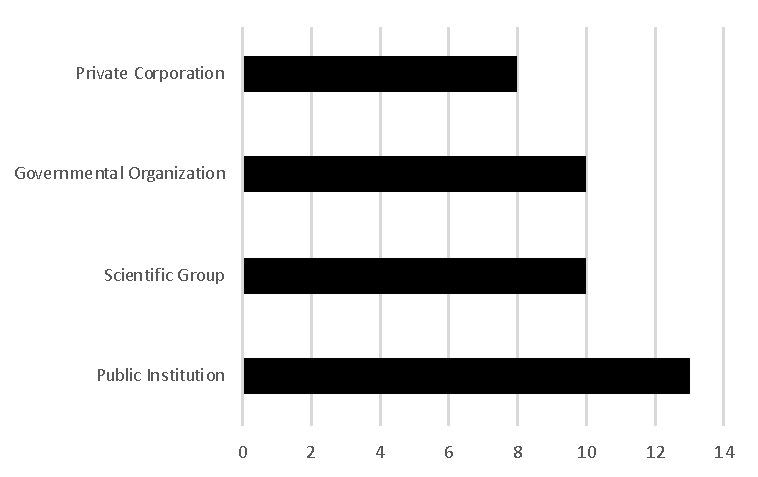
\includegraphics[scale=0.7]{./img/gcorptype}
\end{center}
\caption{types of organizations involved in the grey-literature, a majority of public organizations are involved.}\label{g1}
\end{figure}

The primary sources we reported offer a diverse statistical distribution over the last 20+ years. Figures from \ref{g1} to \ref{g3} outline statistical descriptors for the elicited grey literature while Figures \ref{w1} to \ref{w3} offer a similar insight into white literature. More specifically, Fig. \ref{g1} outlines the types of organisations who conducted the research reported in our primary studies, ranging from private corporations (e.g., Kaspersky labs) to public institutions (e.g., non-governmental organizations and boards), who cover for the majority of our sample. Further on, Fig. \ref{g2} provides a timeline reflecting a linear increase in interest over the phenomenon between the oldest (2006) and newest (2018) article we analysed while Fig. \ref{g3} provides a deeeper insight into the types of evaluations conducted in the grey-literature in question, with a striking majority of experience reports being used as basis for argument.

\begin{figure}
\begin{center}
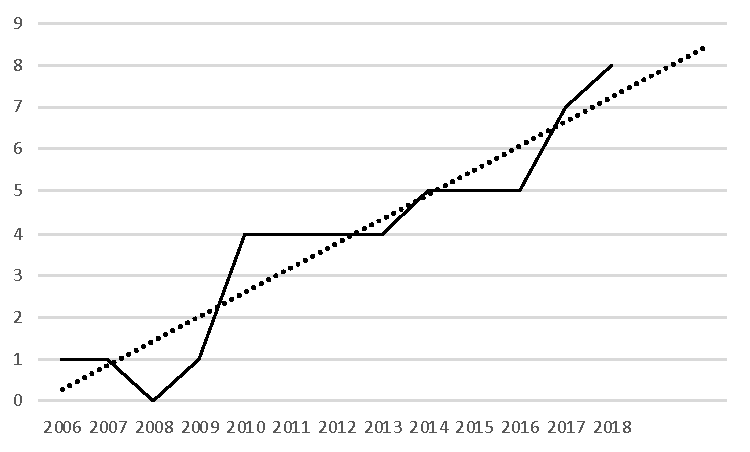
\includegraphics[scale=0.7]{./img/gtimeline.pdf}
\end{center}
\caption{increase of interest over the topic; a linear increase is reported.}\label{g2}
\end{figure}

\begin{figure}
\begin{center}
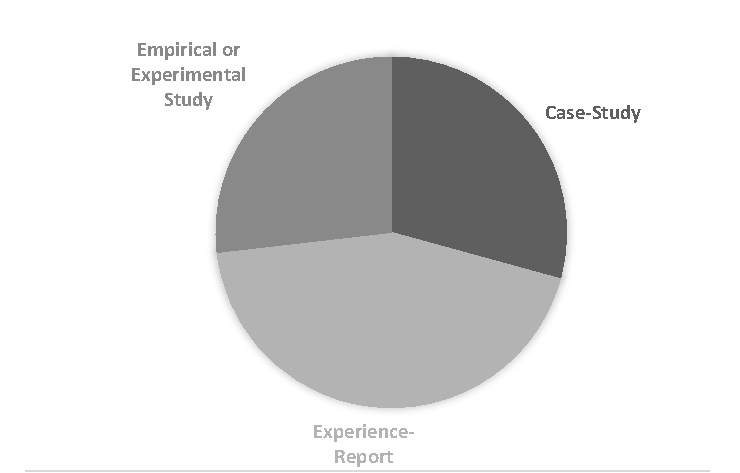
\includegraphics[scale=0.75]{./img/gtypeeval.pdf}
\end{center}
\caption{types of evaluation involved in the grey-literature; experience reports are the striking majority.}\label{g3}
\end{figure}

On the white-literature front, Fig. \ref{w1} offers an overview of the types of studies reported in literature, with a majority of case-studies being targeted for further research.

\begin{figure}
\begin{center}
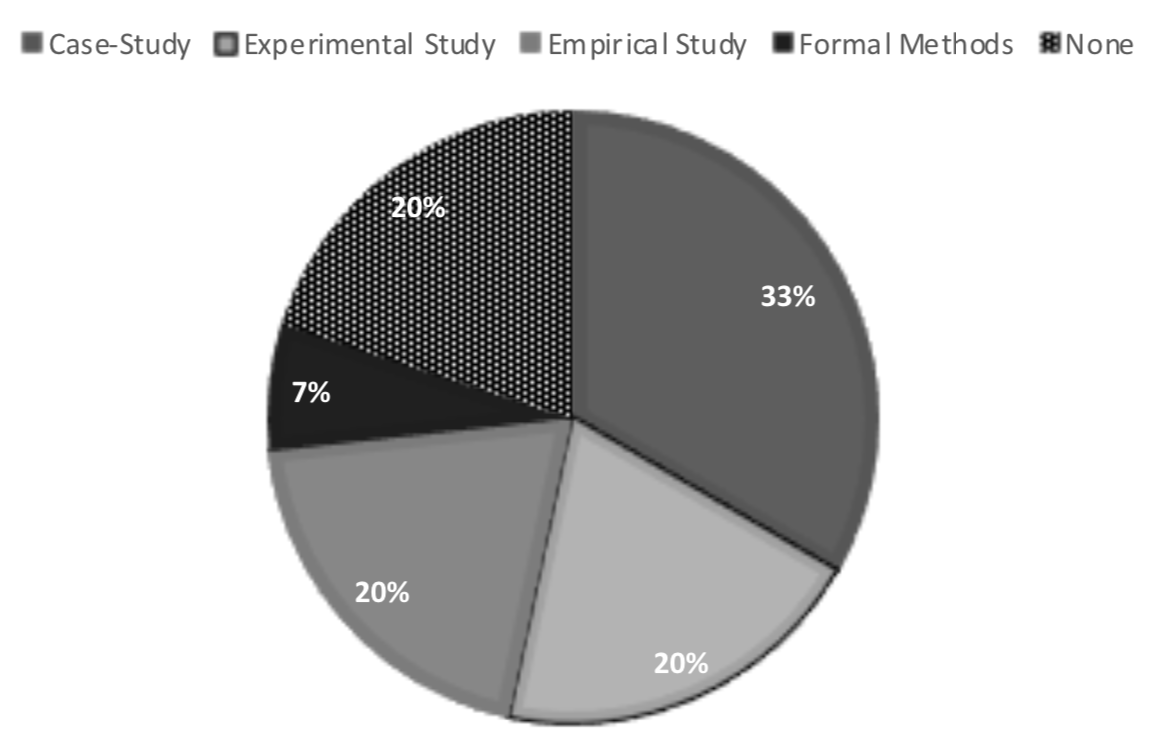
\includegraphics[scale=0.5]{./img/weval.png}
\end{center}
\caption{types of studies conducted in white-literature; case-studies are targeted the most.}\label{w1}
\end{figure}

Beyond the types of studies, Figures \ref{w2} to \ref{w3} offer an overview of the topic interest --- which reflects some mixed trends --- and the typical venues, with a striking preference for conferences --- which are typically more divulgative in nature.

\begin{figure}
\begin{center}
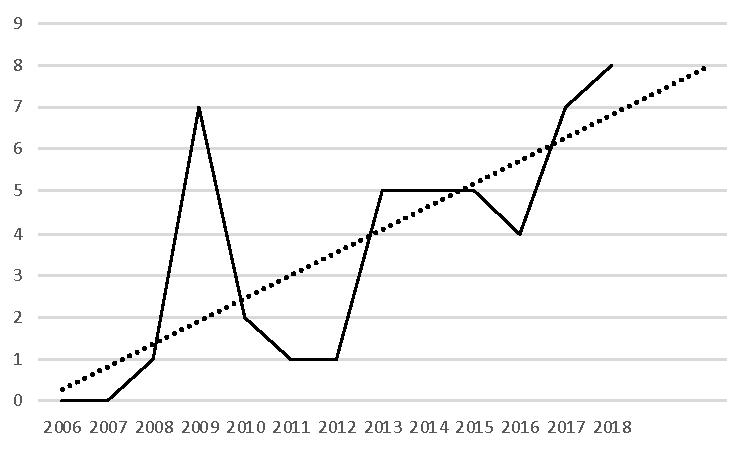
\includegraphics[scale=0.6]{./img/wtimeline.pdf}
\end{center}
\caption{a linear trend is present in white-literature as well; however, mixed but rising interest is reported over the years.}\label{w2}
\end{figure}

\begin{figure}
\begin{center}
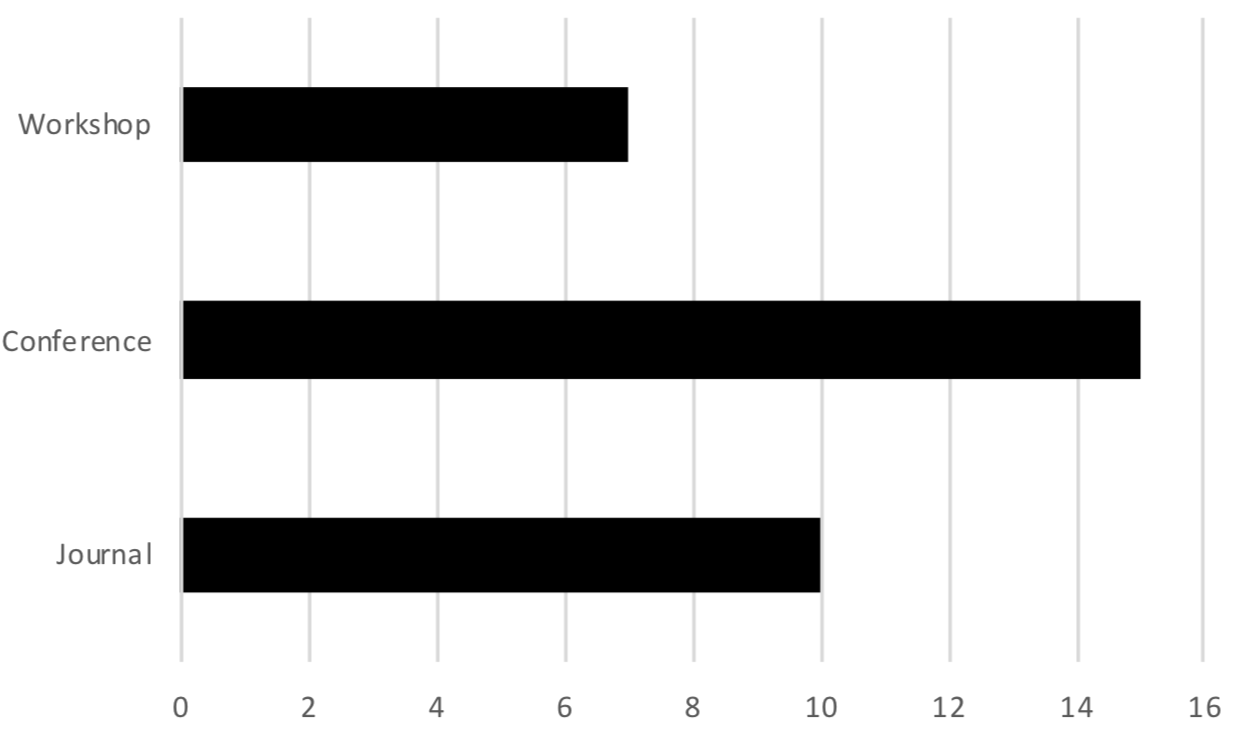
\includegraphics[scale=0.4]{./img/wvenue.png}
\end{center}
\caption{venues selected for publication; the strong preference for conferences or workshops as opposed to journals reflect an emerging discipline.}\label{w3}
\end{figure}

Overall, the statistics offer a not-so-comforting picture. The field seems in an emerging phase, with mixed-feelings or forming interest, typically disseminated in conferences but discussed over case-studies (in white) and/or from experience reports (in grey literature). 

Finally, as an overview of the thematic coding that we adopted to elicit answers for our research questions, Fig. \ref{codescount} offers a quantitative overview of the core concepts discovered as part of our analysis (Definition of codes is provided). The figure highlights that most of the literature we analysed focuses on discussing specific detection \emph{methods} for \emph{criminal activity types}, as opposed to providing holistic methods for the discovery of cybercrime. Moreover, from a quantitative perspective, we highlight that  \emph{website appearance} and their degree of (software) \emph{security} are major indicators for risk assessment. The next sections offer more detail on the results of our study.

\begin{figure}
\begin{center}
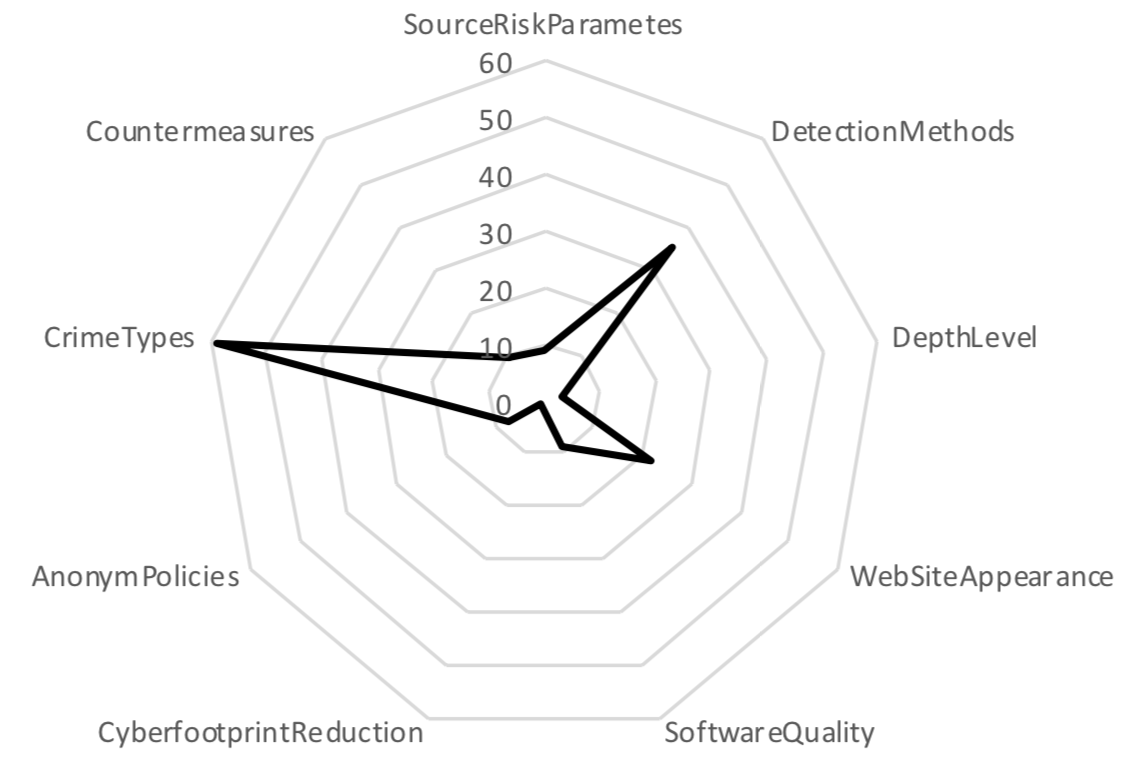
\includegraphics[scale=0.4]{codescount.png}
\end{center}
\caption{Count of occurrences for core-concepts across our dataset, normalized on a percentile scale.}\label{codescount}
\end{figure}

\subsection{Cybercrime Threat Intelligence: A Surface-Web Taxonomy}

Figure \ref{taxo1} outlines the result of our thematic coding as applied to literature discussing or targeting analyses on the \emph{surface} web only.

\begin{figure}
\begin{center}
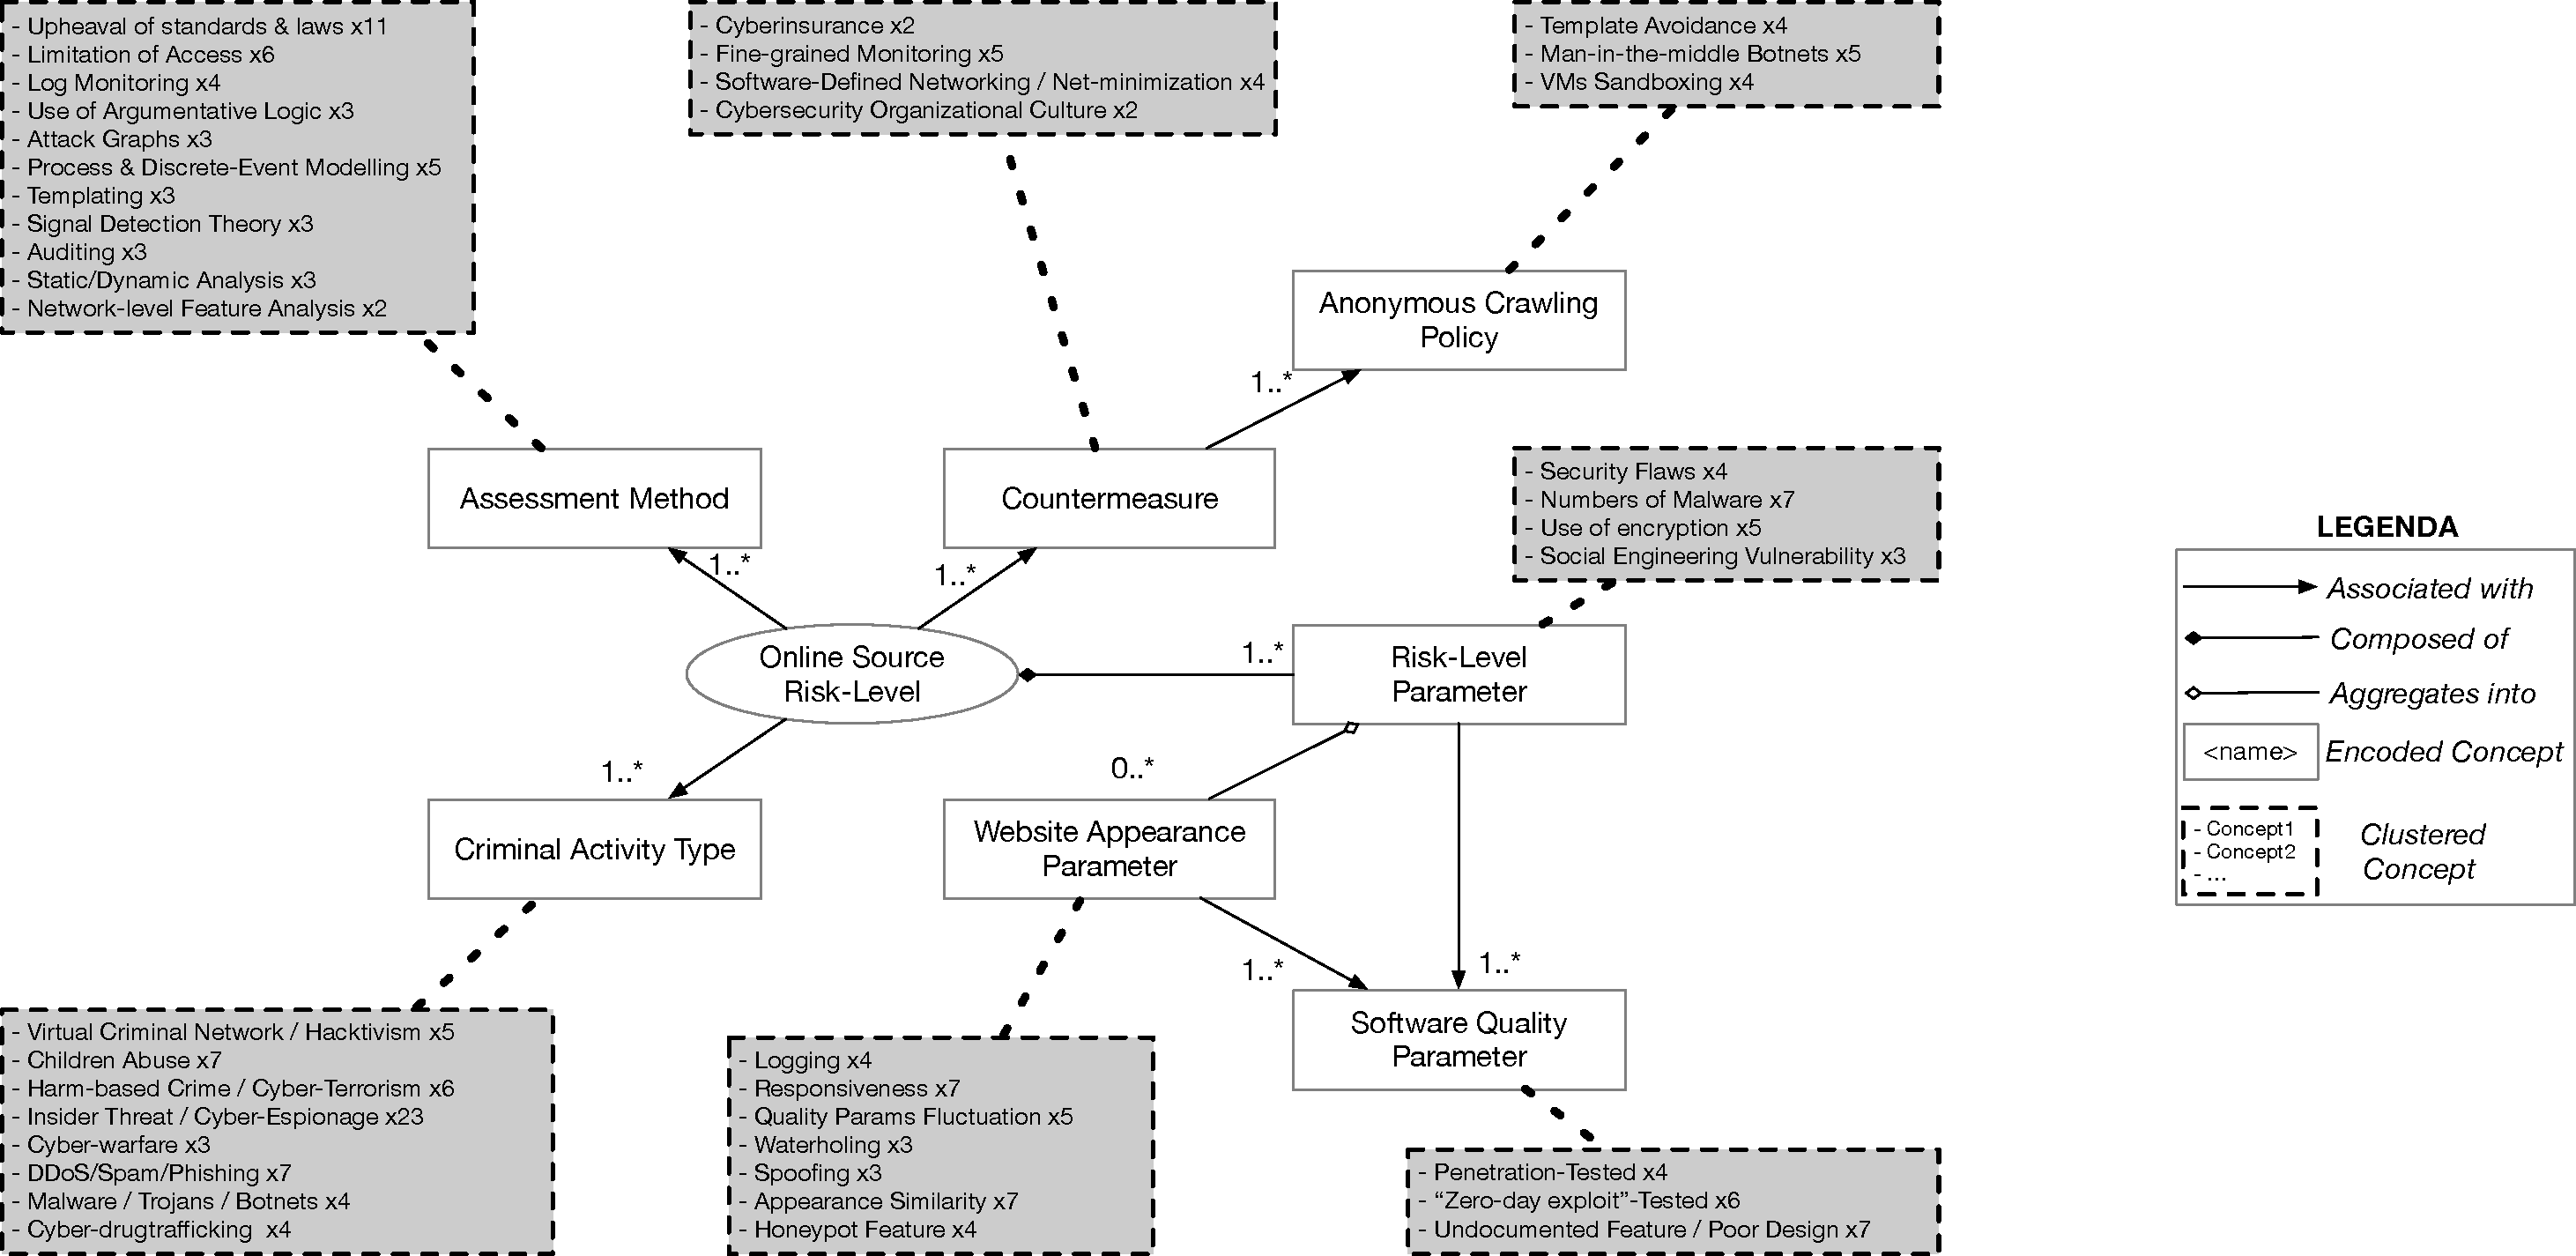
\includegraphics[scale=0.3]{./img/taxo1.pdf}
\end{center}
\caption{A taxonomy of cybercrime threat intelligence for the surface web.}\label{taxo1}
\end{figure}



The results are articulated using a simple UML-like model structured using the core-concepts (inner-most, white boxes on Fig. \ref{taxo1}) emerging from our thematic coding, namely: (a) \emph{assessment methods} --- these are the methods, techniques or tools discussed in the state of the art to address cybercrime threat intelligence; (b) \emph{countermeasures} --- these are the methods and measures that can limit the damage connected to cybercrime, as discussed in literature; (c) \emph{anonymous crawling policy} --- these are the techniques and policies that can limit the detection risk of conducting cybercrime threat intelligence in the open; (d) \emph{risk-level parameters} --- these are indicators for increased risk of specific cybercrimes; (e) \emph{web-site appearance parameters} --- these are ``hints" that previous research identifies as a certain factor indicating that a web source is hosting a specific criminal activity; (f) \emph{software-quality parameter} --- these are software-related quality metrics (e.g., increased throughput or reduced responsiveness) that indicate or are connected to a specific criminal activity being perpetrated; (g) \emph{criminal activity type} --- these are the actual criminal activities being carried out.

The outer-most, grey-colored boxes on Fig. \ref{taxo1} outline what we reported from literature, with a frequency cut-off of 3 recurrences over 3 primary studies from *both* grey and white literature, meaning that concepts, techniques, tools and methods discussed less than 3 times and published or discussed before 2018 were not reported for the sake of space. 

In the following, we flesh-out the results from Fig. \ref{taxo1} in the same order as the core-concepts were outlined in the text above; resulting concepts appear in \emph{italics} in the descriptive sections. It should be noted that, from this point forward, no distinction is made between grey or white literature to avoid any bias in the exposition of the results.

\subsubsection{Assessment Methods}

From a policy perspective, literature remarks that the use of \emph{standards and laws} is the single most-used risk assessment method against cybercrime activity; for example, several articles in both grey and white literature remark that the Gramm-Leach-Bliley Act (GLBA) \cite{Chen2004c} or the Fair Credit Reporting Act (FCRA) \cite{Hoofnagle2013} offer the technical and legal basis to establish the perpetration of online financial crimes of multiple types. In over 30\% of our sample, similar legislations (including GDPR in more modern instances) are suggested as tools in their own right to be used against cybercrime of a more shallow and evident nature in the surface web. Furthermore, several experience reports and case-studies elaborate on the use of \emph{limitation of access} or access-control blacklists as a method to establish and limit the involvement with cybercrime. More specifically, tools and approaches such as SquidGuard~\footnote{\url{http://squidguard.mesd.k12.or.us/}} offer a basis to share and adopt lists of sites hosting criminal activities to be avoided. 

From a more technical perspective, \emph{log monitoring} is highlighted as the most obvious cybercrime risk detection and avoidance method. For example, Mataracioglu et al. \cite{MataraciogluOH15} report on a cybercrime and cybersecurity framework which harnesses log monitoring to detect and avoid social engineering tactics often employed as part of cybercrime. A similar argument is made for the use of log monitoring in several articles from the proceedings of the federated conference on Data Privacy Management, Autonomous Spontaneous Security, and Security Assurance \cite{2014-8872}. In  these venues, log monitoring is combined with \emph{attack graphs}, a formalism built on top of log monitoring techniques that can elicit social engineering attacks by dissecting the connected social engineering threats and vulnerabilities \cite{BeckersKY14}. Similarly to attack graphs, log monitoring and similar runtime threat detection and avoidance activities combine \emph{process modelling/mining} and \emph{argumentative logic}. For example, Bouyahia et al. \cite{BouyahiaICCA14} introduce a metrics-based technique to assist the detection and avoidance of security threats using reasoning systems which incrementally figure out ongoing attacks --- while ontology-based approaches are highlighted in the paper, the authors also remark on the potential to combine a more data-driven machine-intelligence approach. 



From a process mining and modelling perspective, the techniques of \emph{discrete event modelling} dating back to '97 and to Harel and Gery seminal work on object state charts \cite{HarelGery1997}, to signals-detection theory \cite{Green1989} and signals intelligence \cite{MaLPLWZL18} applied to \emph{static/dynamic networks traffic analysis}, and ending up with a recent work focusing on terrorist attacks by Gabriels et al. \cite{abrielSBSGM17}.

Overall, on the one hand, the state of the art results as *very* domain-specific (e.g., terrorist attacks \cite{abrielSBSGM17}, insider threats \cite{Blackwell2009}) mostly based on \emph{templating} of crimes --- that is, offering a standardized format for the perpetrated crime and matching that format onto available data --- and with little generalizable approaches. 

On the other hand, the last two approaches we reported as recurrent, namely, \emph{auditing} and \emph{network-level feature analysis} offer theoretical bases for generalisability. More specifically, cybercrime auditing entails providing for strategic checking of organisational and technical infrastructures by randomly selecting a cybercrime type, instrumenting the type and purposefully targeting the organisational and technical infrastructures with it to evaluate the target infrastructures' vulnerability to it~\footnote{\url{http://m.isaca.org/knowledge-center/research/researchdeliverables/pages/cybercrime-audit-assurance-program.aspx}}. With respect to the auditing technicque highlighted above, Chang et al. \cite{ChangVWL13} offer an in-depth overview of malware-based crimes which is offered as a basis for targeted auditing.

Finally, with respect to network traffic analysis, several approaches reported in literature offer feature-based (social) network analysis \cite{ORiordanFN16} as well as feature engineering and analysis techniques aimed at establishing precursors of social engineering, most notably from our dataset the works by Vidal et al. \cite{VidalC17} or Garibi et al. \cite{abs-1201-0949}.

\subsubsection{Countermeasures}

As previously specified, with the term \emph{countermeasure} we identify the ability to foresee and enact preemptive or corrective action against a specific cybercriminal activity. On one hand, most of the grey literature highlights the need to conduct business-level impact assessment and incident management, for example, the report of the Australian Government \cite{ring2017data} remarks that businesses need to be arrange, quoting from the original document, specific \emph{``actions taken as soon as an attack or breach has occurred to determine the (1) depth of its effect on the business, (2) your ability to recover, and (3) affect the likelihood of future breaches"}. Several proactive actions have been introduced. For example, Baer et al. discuss several approaches to Cyberinsurance \cite{BaerP07} and similarly, earlier works by Meland et al. \cite{MelandTS15} establish the ways in which cyberinsurance actions can be planned as part of corporate governance and towards the reduction of cyberthreats risks.

From a more analytical perspective, several technical countermeasures were proposed, mostly along the lines of fine-grained monitoring of IT assets and business processing; more specifically
Ma et al \cite{Ma2012}, as early as 2012, offer a ightweight framework for monitoring public clouds which is outlined as a potential solution for mitigating cyberthreats, as long as an appropriate incident response organisational structure and culture \cite{ChangL07,TangLZ16} is also in place whereupon a threat does manifest. Later works offer prototypical solutions where cloud and IT infrastructures monitoring is combined with real-time applications security \cite{CoppolinoDFR14}. Still on a technical perspective, acting as a countermeasure for cybercrime is the use of software-defined networks (SDNs) as well as virtual-networks functions (VNFs), that is, harnesssing with programmable/controllable software the responsibility of handling specific network functions that run on one or more virtual machines. In this specific domain, the survey by Hayward et al. \cite{scotthayward2013sec} offers an overview of the practices in SDNs which can be used to attain software-controlled granular cybersecurity and safety.

\subsubsection{Anonymous Crawling Policies}

In terms of maintaining anonymity while performing cybercrime detection or avoidance tasks across an organizational structure, much research has devoted to the use and refinement of Bots and botnets dedicated to detect social engineering attacks or perform anonymous analysis. For example, the works by Lauinger et al. \cite{LauingerPBK10} and subsequent trials by the US Chamber of commerce contained in their whitepaper\footnote{\url{https://www.uschamber.com/CybersecurityEssentials}} remark that \emph{``an acceptable-use policy for the use of information resources and IT systems [needs] for example, confidential or sensitive business information not to be posted by employees on social networking sites such as Facebook or MySpace [...]"}; the aforementioned actions were experimented upon with the usage of policy-driven bots to perform counterinsurgency of amended actions. Likewise the survey by Chang et al. \cite{ChangVWL13} offers an overview of several approaches along the lines defined above wherefore web-based malware is detected, risk-assessed, avoided using on-purpose, policy-driven botnets. 

Finally, in terms of anonymity during detection phases for cybercriminal activity, the use of Virtual-Machine sandboxes is often referred to as the only viable mechanism \cite{ChangVWL13} but several recent works show the endurance of specific attacks or other masqueraded cybecriminal activity such as the S\$A and similar shared-cache attacks \cite{ApececheaES15} against a sandboxing approach.

\subsubsection{Risk-Level Parameters}

This section showcases the few parameters reported in literature which are commonly known to increase the risks of cybercriminal activity being perpetrated in targeted online sources. An outstanding number of whitepapers and governmental reports highlight the presence and proliferation of several risk-related parameters; most notably, as noted in the US Chamber of commerce whitepaper about cybercrime\footnote{\url{https://www.uschamber.com/CybersecurityEssentials}}, ``[actions need to be taken to] root out security flaws in computer programs and to counter cyberattacks by ``bad" hackers, or cybercriminals", hence indicating the presence and extent of security flaws (of which, the number of Malware is an established minimum, as noted by Rahul et al. \cite{Rahul} and several others \cite{Caballero12}) in the code of online sites as a probable factor of risk in establishing high-threat sources. Finally, the haphazard use (or lack thereof) of encryption across online source functions has been established to lead to cybercriminal activity, most notably in the roadmap defined by Kieseberg et al. \cite{KiesebergSR15}. More specifically, the lack of encryption is often connected to the use of specific social engineering activities being perpetrated in online sources, which themselves are functional to cybercrime \cite{Gharibi}. On this latter front, that of social engineering vulnerabilities specifically designed to accomodate for cybercriminal activity, several authors such as Vidal et al. \cite{VidalC17} remark on the necessity to conduct scenario-based situational crime prevention, e.g., using evolutionary computing and social predictive analytics --- the work along these lines has mostly concentrated on elaborating more or less complete cyberforensics ontologies for the purpose of knowledge representation and reasoning about cybercriminal investigation in a scenario-based fashion \cite{ParkCK09}.

\subsubsection{Software Quality Parameters}

The necessity to establish security as a software quality parameter to decide whether an online source bears risk of cybercriminal activity finds agreement in ~90\% of both grey and white literature alike. More specifically, the quality of software security is established around three axes: (1) whether the online source bear signatures and certificates of successful penetration-testing \cite{franklin}; (2) whether the online source has been certified against morphisms \cite{li06ieee,GuptaR18} of known zero-day exploits \cite{Danforth11,BilgeD13}; (3) finally, whether the online source bears undocumented software features and/or the indications of poor design (e.g., technical debt, etc.) \cite{NordOSSK16}.

\subsubsection{Website-Appearance Parameters}

In terms of website appearance, the literature we analysed identifies seven features as indicative pre-conditions to cybercriminal activity: (1) the lack of logging as well as software features for forward error correction, site responsiveness as well as other constructs that measure all graph-theoretic properties of the darknet (e.g., see Griffith et al. \cite{GriffithXR17}); (2) variable responsiveness rates from the online source \cite{} (3) a heavy fluctuation of the overall software quality parameters (e.g., language clarity, documentation, feature stability, etc.) for the online source, oftentimes detected thorugh anomaly detection or linear-time temporal logics, as seen in Almukaynizi et al. \cite{AlmukayniziPSSS18}; (4) the existence of waterholing features, defined by Trendmico\footnote{\url{https://www.trendmicro.com/vinfo/in/threat-encyclopedia/web-attack/137/watering-hole-101}} as areas of the site which are uncontrolled, uncontrollable, or never improved overtime by site maintainers \cite{KhanIJKBIES}; (5) the presence of spoofed information mismatches detectable through online fact-checking, an approach to this is presented in Nunes et al. \cite{NunesSS18}; (6) a high degree of appearance similarity with respect to other known online sources \cite{GhoshPYND17,MartineR05}; (7) finally, honeypot features most predominantly the length and target of the redirection chain upon any navigation request from the source, since almost 68\% of our sources from white and grey literature studies observe that malicious landing sites almost always have unusually long redirection chains toward malware distribution sites \cite{ChangVWL13}.

\subsubsection{Criminal Activity Types}

Lastly, the risk assessment of online sources can be supported by focusing the identification of the risk using combined measures of likelihood for reported criminal activity types \cite{Elstob74}. This section outlines and discusses all criminal activity types we reported in literature. As previously remarked, we report in this section the crime types reported at least 3 times in at least 3 papers from both grey and white literature (i.e., at least 6 papers in total), later in Sec. \ref{disc} we discuss emerging crime activity types reported in more recent literature. Overall, the literature on cyberthreat intelligence focuses around 7 criminal activity types, namely: (1) Virtual Criminal Network / Hacktivism Groups --- these reflect, on the one hand, crime networks dedicated to regular crime activity (e.g., drug trafficking) exploiting online means \cite{HanWCMZ17} and, on the other hand, forms of cyber-activism (i.e., Hacktivism), where cyber attacks are ideologically motivated and have primarily a demonstrative intent, like damaging the image of the target and/or causing a temporary malfunctioning of the attacked ICT systems \cite{sureka2010mining}; (2) Children Abuse --- these reflect sites exploiting minors for malicious intents and purposes, including and not limited to humans trafficking \cite{HanWCMZ17}; (3) Harm-based Crime / Cyber-Terrorism --- these activities are usually ideologically motivated, as outlined by Gordon \cite{GordonF02}, and uses exploitations of systems vulnerabilities with the intent of influencing a state or an international organization \cite{VeerasamyG15};  (4) Insider Threat / Cyber-Espionage --- these activities focus on the exploitation of organizational insiders \cite{Rocha15a} for the purpose of information trafficking and intelligence, with works ranging from classification of threat intelligence risks \cite{SantosNYKLWOJC12} to stream reasoning technology for live detection of leaks \cite{ParveenMWETHK13}. Oftentimes such cyber-espionage is functional to (5) Cyber-warfare --- these activities focus on operations carried out in the cyber domain with the purpose of achieving an operational advantage of military significance, with a full report from the US Military intelligence \cite{Cordesman2002} as a seminal work; (6) DDoS/Spam/Phishing --- similarly to cyber-espionage Distributed Denial of Service \cite{Kandula05}, Spam or Phishing criminal activities are connected to crimes against critical infrastructures \cite{setola2016critical} - for example attacks affecting the integrity of data or information systems used in Supervisory Control and Data Acquisition Systems (SCADA) could be used to overload power grids, block communications and financial transfers, etc; (7) cyber drug-trafficking --- these activities focus on the stockade, movement, production, and reselling of illegal substances, wit early works focusing on identifying the extent and properties of the collaboration networks lying beneath \cite{Wood17}.

Overall for the above crimes all have been reported in connection to software-based electronic threats, vulnerabilities, and attacks where Malware (including ransomware and similar malware aiming explicitly at financial gains), Trojans, or Botnets play an instrumental knowledge-gathering and insurgency role, with latest works on this research stream discussing the architectural properties of malware altogether, e.g., Lakhotia et al. \cite{LakhotiaB17}.


\subsection{Cybercrime Threat Intelligence: A Taxonomy for Deep- and Dark-Web}

Beyond the previously defined taxonomy addressing the surface web, this section discusses the approaches, countermeasures, indicators for Cybercrime Threat Intelligence in the deep- and dark-webs. The taxonomy in question (see Fig. \ref{taxo2}) shares overlaps with its surface web counterpart (see Fig. \ref{taxo1}), specifically in the criminal activity types and countermeasures thereof (see the greyed boxes with ``.*" symbol).

\begin{figure}
\begin{center}
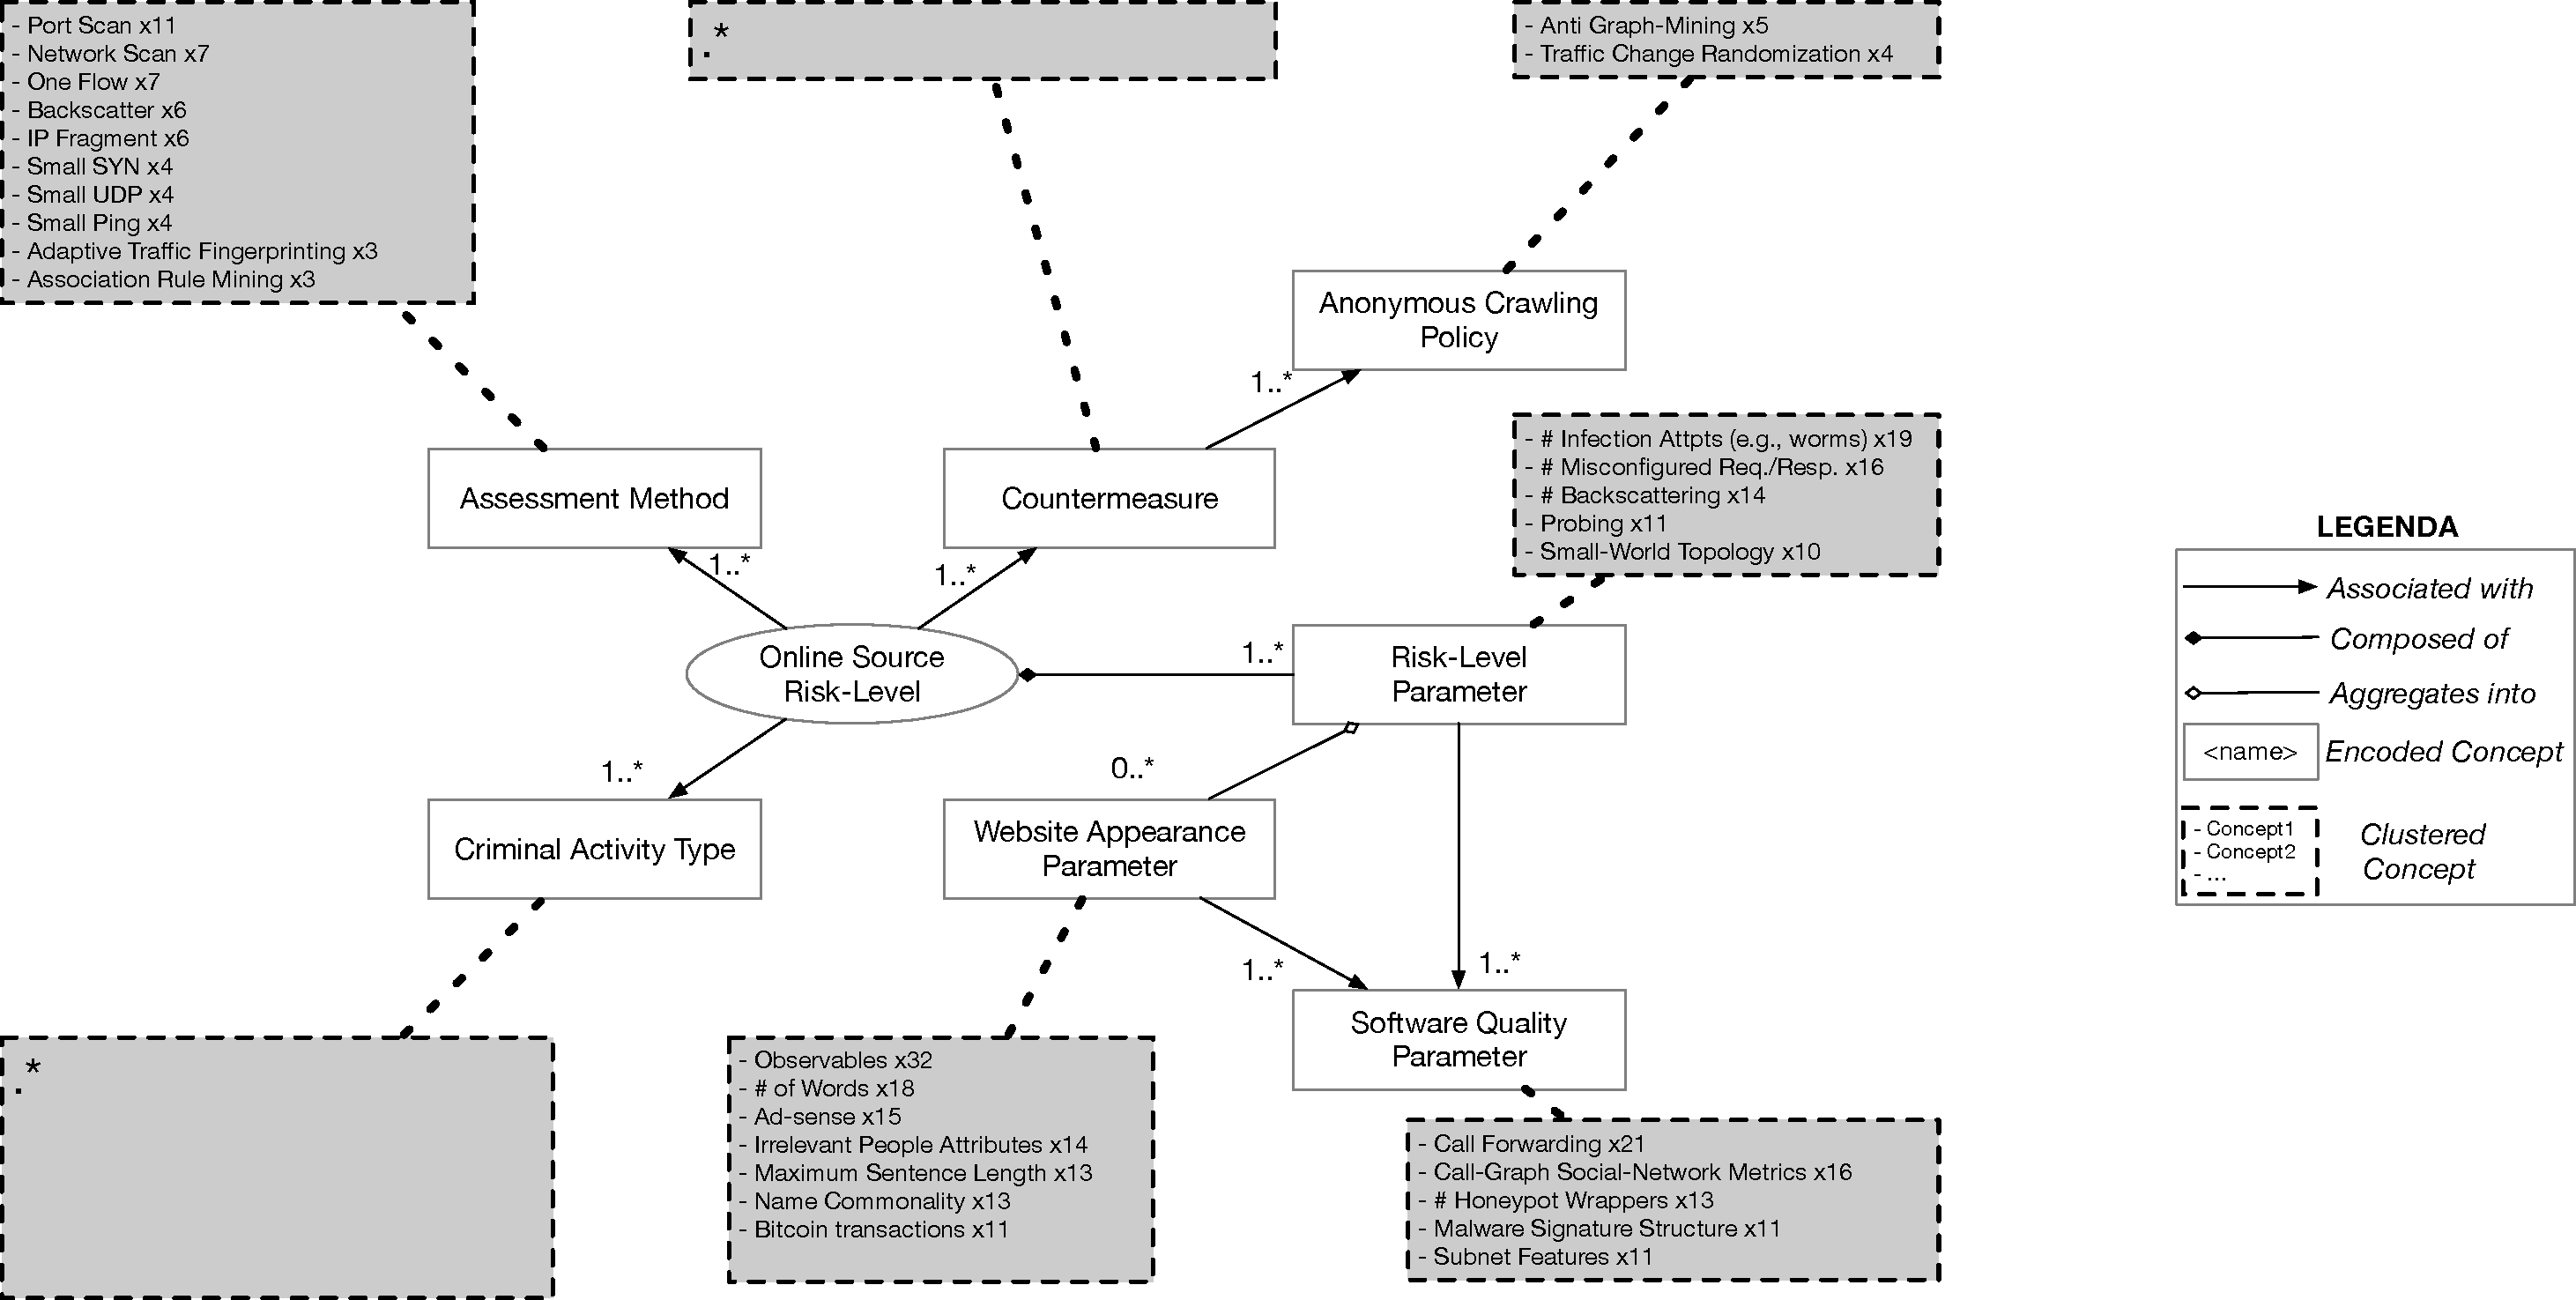
\includegraphics[scale=0.3]{./img/taxo2.pdf}
\end{center}
\caption{A taxonomy of cybercrime threat intelligence for the surface web.}\label{taxo2}
\end{figure}


\subsubsection{Assessment Methods}

TODO\\

\subsubsection{Anonymous Crawling Policies}

TODO\\

\subsubsection{Risk-Level Parameters}

TODO\\

\subsubsection{Software Quality Parameters}

TODO\\

\subsubsection{Website-Appearance Parameters}

TODO\\

\subsection{Cybercrime Threat Indicators: Topic Modelling Results}

In this paragraph we are now going to discuss the results of our Topic Modelling Analysis on our set of papers. As previously stated, we used Latent Dirichlet Allocation (LDA) to highlight the most relevant themes in our textual data, however before applying LDA we pre-processed our text. The pre-processing phase aims at improve our final results and consist of: \emph{i} removal of unwanted chars, numbers and symbols (like words smaller than two chars), \emph{ii} removal of stop-wars, \emph{iii} lemmatization in order to reduce any given word to its root form thereby reducing multiple forms of a word to a single word.
After the pre-processing phase we apply LDA method for visualizing and interpreting topics, the method we used is the one described in \cite{W14-3110} called \textbf{LDAvis} and based on the work of Chuang et. al in \cite{Chuang:2012:TVT:2254556.2254572}. The paper, moreover, gives the instructions to read the diagrams we plotted, however, below continue with a small recap about how to interpret our diagrams. 
On the left side of our figures we have a recap of our topics, each of the circle represent a topic and how prevalent it is, moreover if the circles are overlapping each other means that those topics have common terms. Into each of this circle are sorted our terms in a decreasing order of prevalence.
The right panel of our results depicts a horizontal barchart whose bars represent the individual terms that are the most useful for interpreting the currently selected topic on the left. The overlaid bars represent both the corpus-wide frequency of a given term as well as the topic-specific frequency of the term \cite{W14-3110, Chuang:2012:TVT:2254556.2254572}. The $\lambda$ slider allows to rank the terms according to term relevance. Moving the slider allows to adjust the rank of terms based on much discriminatory (or ``relevant'') are for the specific topic, we fixed the $\lambda$ at 0.8.\todo{suggested value is 0.6, however nothing change with the results}

Here below we are now going to discuss our results of our topic modelling analysis. For each analysis in Fig.~\ref{fig:topicmodelling_1}, Fig.~\ref{fig:topicmodelling_2}~and Fig.~\ref{fig:topicmodelling_3} \todo{missed dark and deep web analysis} we build a table where we summarize and discuss the most relevant terms related to the cybersecurity field. 

\subsubsection{Topic modelling results for Surface Web}

In Table~\ref{tab:topicmodelling_1} we have the list of words from \textit{Topic~1}. 


%%%%%%%%%% TABLE topic 1 %%%%%%%%%%%%%%

\begin{table}[H!]
%\small
%\resizebox{\textwidth}{!}{%
\scalebox{0.8}{
\begin{tabular}{@{}lll@{}}
%\begin{tabular}{p{0.12\textwidth}p{0.8\textwidth}p{0\textwidth}}
\toprule
\textbf{Terms} & \textbf{Score} & \textbf{} \\ \midrule 
\rowcolor[HTML]{EFEFEF} 
System & 40 & \begin{tabular}[c]{@{}l@{}}
The system can receive different type of attacks. The operating system of a PC, if not properly\\ maintained, can easily be the target of virus, worm, malware, spyware and other cyberthreat\\ attacks. In order to protect the system of a private user is important to have an antivirus\\ and keep the system updated. In a private company is important to educate the \\ employee to do not use distrusted applications and to use strong passwords in order to protect\\ personal information. An attack to the system can involve a loss of personal data, a destabilization  \\ of the running processes of the system and the forward of private information to third parties.\end{tabular} \\
\rowcolor[HTML]{FFFFFF} 
Vulnerability & 27 & \begin{tabular}[c]{@{}l@{}} Techopedia defines the therm \textit{vulnerability} as cyber-security term that refers to a flaw in a system\\ that can leave it open to attack. A vulnerability may also refer to any type of weakness in a computer\\ system itself, in a set of procedures, or in anything that leaves information security exposed to a\\ threat \cite{techopedia}. Some computer vulnerabilities include bugs, weak password, outdated operating \\ system, OS command injection, download of pirate software. Computer users and network personnel\\ can protect computer systems from vulnerabilities by keeping software security patches up to date, \\moreover, to better increase our cybersecurity, is important to use programs like firewall, anti-virus,\\ web URL filtering and avoid thye download of pirate software.\end{tabular}\\ 
\rowcolor[HTML]{EFEFEF} 
Threat & 27 & \begin{tabular}[c]{@{}l@{}}  We live in a hyperconnected world, half the world's population is interconnected through Internet\\ and 125 billion of IoT devices are expected by 2030 to be connected. All this complexity along with\\ constantly evolving nature of cybersecurity threats is leading to more breaches and cyber attack\\ threats. Threats are potentials for vulnerabilities to turn into attacks on computer systems, networks,\\ and more. They can put individuals' computer systems and business computers at risk, so\\ vulnerabilities have to be fixed so that attackers cannot infiltrate the system and cause damage.\\ Threats can include everything from viruses, trojans, back doors to outright attacks from hackers \cite{techopedia}.\end{tabular}\\ 
\rowcolor[HTML]{FFFFFF} 
Malware & 17 & \begin{tabular}[c]{@{}l@{}} Malicious software (MALWARE) is one of the most common cyber threat attack. A MALWARE is\\ any software that does harm to the system, such as a virus or spyware. There are a lot of different \\ versions of MALWARE: virus, trojan, rootkit, worm, spyware and adware, all of them with different\\ characteristics but with the same purpose. The aim of all this malicious software is to steal private \\ information from the victim's PC, profile the habits of the victim user, use the attacked machine as a\\ zombie for network attacks.\end{tabular} \\ 
\rowcolor[HTML]{EFEFEF} 
Software & 17 & \begin{tabular}[c]{@{}l@{}} As software prices increase, many users turn to installing bootleg copies, or pirated ones. According \\ to the study in \cite{piracy} 34\% of the downloaded pirated software came bundled with malware that infect\\ the computer once the download is complete or when the folder containing the pirated software is\\ opened. In order to avoid any type of risk, a solution is to use free version of the software or similar\\
software but free or open source. \end{tabular} \\ 
%\rowcolor[HTML]{EFEFEF} 
%Victim & 15 &  \end{tabular}\\ 
\bottomrule
\end{tabular}
}
\caption{Topic analysis results of the first topic in Surface Web.}
\label{tab:topicmodelling_1}
\end{table}




% \begin{table}[h!]
% \small
% \resizebox{\textwidth}{!}{%
% %\begin{tabular}{p{0.10\textwidth}p{0.10\textwidth}p{0.70\textwidth}}
% \begin{tabular}{@{}lll@{}}
% \toprule
% \textbf{Terms} & \textbf{Score} & \textbf{} \\ \midrule 
% \rowcolor[HTML]{EFEFEF}
% Packet & 19 & \begin{tabular}[c]{@{}l@{}} The Denial of Service (DoS) attack is meant to shut down a machine or a network and its services\\ making it inaccessible to the users. The main target of DoS attack are usually  web servers of\\ high-profile organizations such as banking, commerce, and media companies, or government and\\ trade organizations. In general we have two types of DoS attack: flooding services and crashing services.\\ The first is caused by high traffic to the servers that makes the services slow down and eventually stop.\\ In the latter case the DoS attack exploit vulnerabilities in order to let crash the running services or\\ destabilize the system.\end{tabular} \\
% \rowcolor[HTML]{FFFFFF} 
% Website & 19 & \begin{tabular}[c]{@{}l@{}}A website can be the place of cyberthreat attacks if the system behind it is not well updated or if the \\ passwords used by the admin are not strong enough. A compromised website can host different types \\ of cyberthreat attacks. A Phishing website is able to steal passwords and personal information of a \\ user. A website can also be the target of SQL Injection Attack in order to retrieve private information \\ from the database.\end{tabular} \\
% \rowcolor[HTML]{EFEFEF} 
% Network & 13 & \begin{tabular}[c]{@{}l@{}}Network attacks are launched every hour of every day, and they are evolving in complexity and level \\ of danger. WiFi attacks aim at stealing password of a personal network in order to commit illicit actions. \\ The most common attacks to the WiFi network are Fake WiFi Access Points, Evil Twins, and Man in \\ the Middle Attacks all of them in order to intercept the data and steal personal information.\end{tabular} \\
% \rowcolor[HTML]{FFFFFF} 
% Email & 10 & \begin{tabular}[c]{@{}l@{}}The emails are one of the main vehicle of information and data. The Identity Theft attack happen when \\ an attacker is able to gain a handle on the employee's email account. The attacker can then turn into the \\ employee's identity. Phishing Attacks a type of social engineering attack often used to steal user data, \\ including login credentials and credit card numbers. It occurs when an attacker, masquerading as a\\ trusted entity, dupes a victim into opening an email. The recipient is then tricked into clicking a malicious\\ link. Virus as attachment to the email in order to install unwanted software on the PC of the user. Spam\\ email are commonly used in order to deliver Trojan horses, viruses, worms, spyware, and targeted\\ phishing attacks or to bring users on a external website in order to steal private and personal information.\end{tabular} \\
% \rowcolor[HTML]{EFEFEF} 
%  &  &  \\
% \rowcolor[HTML]{EFEFEF} 
%  &  &  \\ \bottomrule
% \end{tabular}
% }
% \caption{Topic analysis results of the first topic in Surface Web.}
% \label{tab:topicmodelling_1}
% \end{table}

%%%%%%%%%%%%%%% ANALIS TOPIC 1

\begin{figure}[H!]
\begin{center}
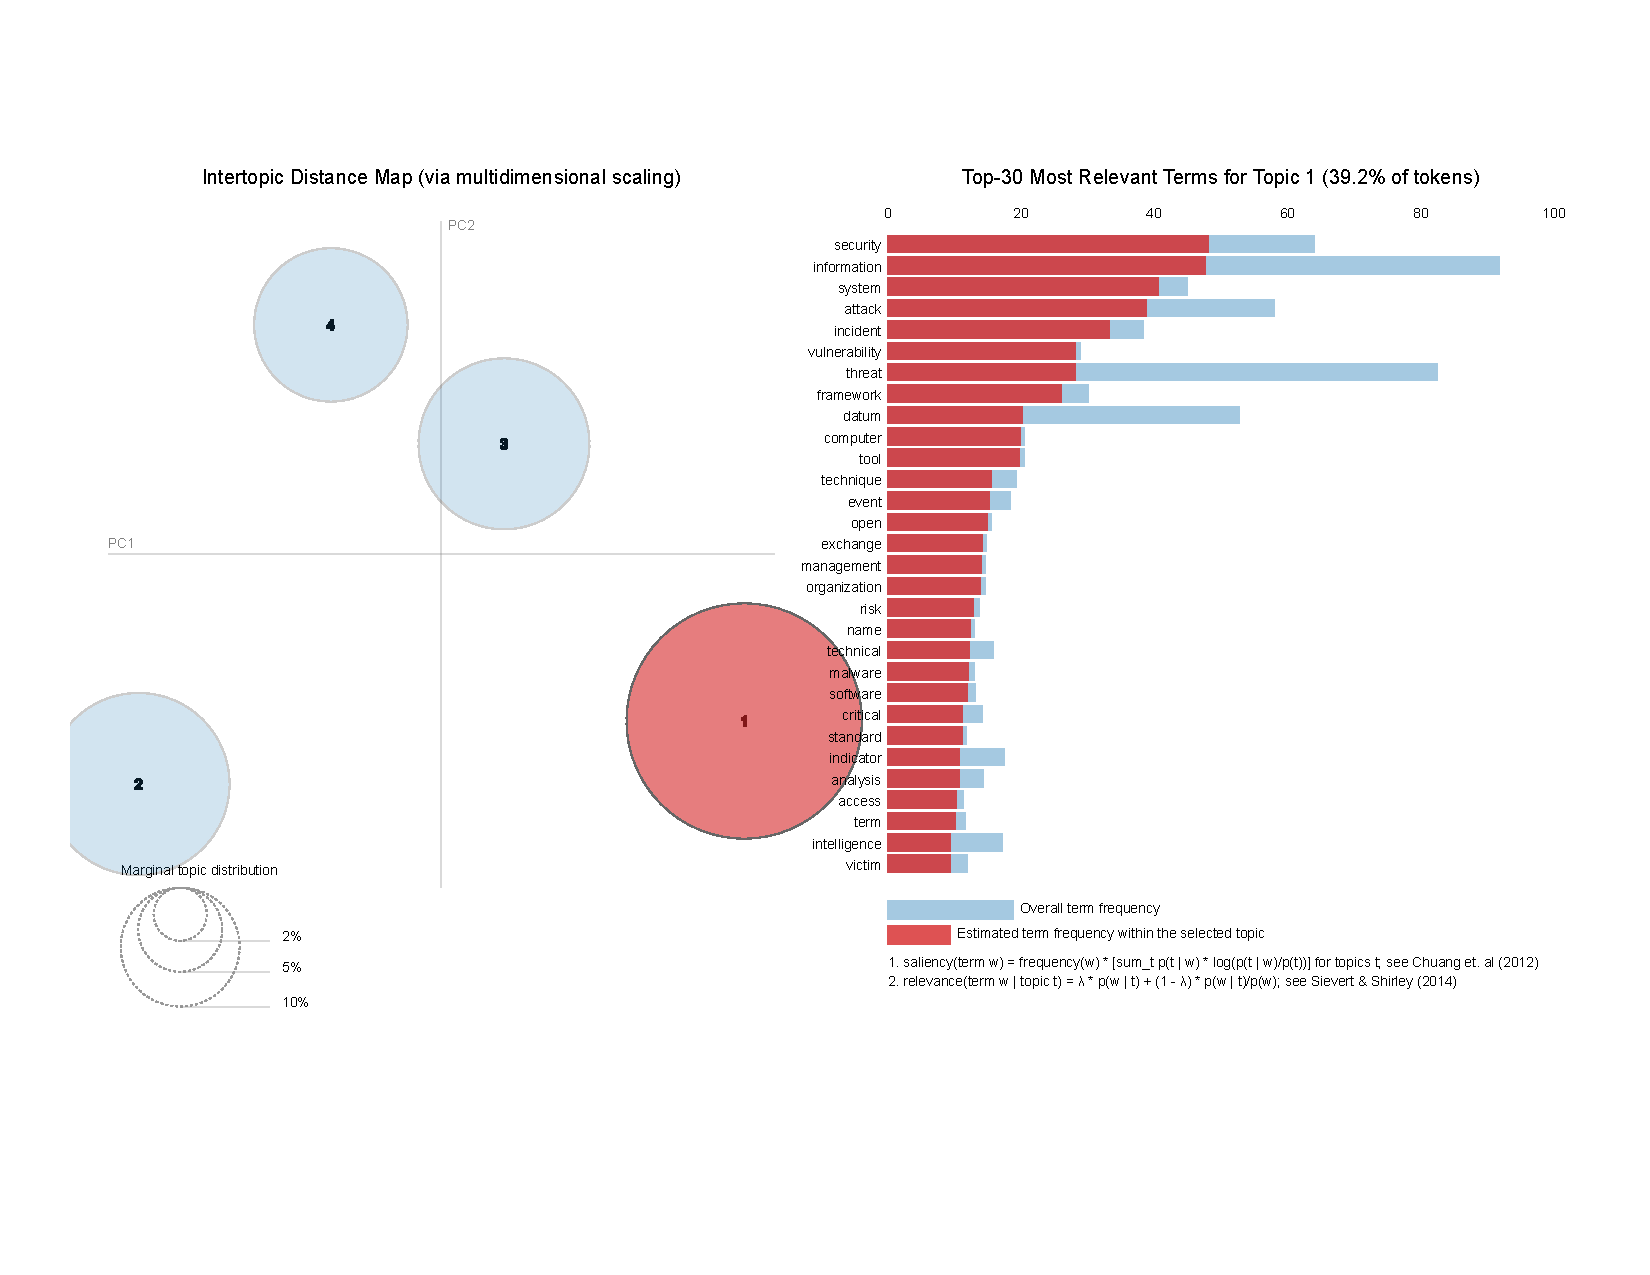
\includegraphics[scale=0.3]{./img/codingALL_topic1.pdf}
\end{center}
\caption{Topic modelling results of the first topic in Surface Web.}
\label{fig:topicmodelling_1}
\end{figure}

%%%%%%%%%%%%%%% %%%%%%%%%%%%%%% 
%%%%%%%%%%%%%%% %%%%%%%%%%%%%%% 
%%%%%%%%%% TABLE topic 2 %%%%%%%%%%%%%%

\begin{table}[h!]
\small
\resizebox{\textwidth}{!}{%
\begin{tabular}{@{}lll@{}}
\toprule
\textbf{Terms} & \textbf{Score} & \textbf{} \\ \midrule 
\rowcolor[HTML]{EFEFEF} 
System & 26 & \begin{tabular}[c]{@{}l@{}}The system can receive different type of attacks. The operating system of a PC, if not properly\\ maintained, can easily be the target of virus, worm, malware, spyware and other cyberthreat\\ attacks. In order to protect the system of a private user is important to have an antivirus\\ and keep the system updated. In a private company is important to educate the \\ employee to do not use distrusted applications and to use strong passwords in order to protect\\ personal information. An attack to the system can involve a loss of personal data, a destabilization  \\ of the running processes of the system and the forward of private information to third parties.\end{tabular} \\
Software & 8 & \begin{tabular}[c]{@{}l@{}}Malicious software (MALWARE) is one of the most common cyber threat attack. A MALWARE is\\ any software that does harm to the system, such as a virus or spyware. There are a lot of different \\ versions of MALWARE: virus, trojan, rootkit, worm, spyware and adware, all of them with different\\ characteristics but with the same purpose. The aim of all this malicious software is to steal private \\ information from the victim's PC, profile the habits of the victim user, use the attacked machine as a\\ zombie for network attacks.\end{tabular} \\
\rowcolor[HTML]{EFEFEF} 
Url & 8 & \begin{tabular}[c]{@{}l@{}}Url is a unique identifier used to locate a resource on the internet. However, often Url's are used to\\ carry unaware users on distrust websites built in order to steal personal information and banking \\ coordinates and passwords. Url's are spread through emails, gaming platforms from OSN (Online \\ Social Networks), SMS and instant messaging platforms.\end{tabular} \\
 &  &  \\
\rowcolor[HTML]{EFEFEF} 
 &  & \\ \bottomrule
\end{tabular}
}
\caption{Topic analysis results of the second topic for Surface Web.}
\label{tab:topicmodelling_2}
\end{table}

%%%%%%%%%%%%%%% ANALIS TOPIC 2

\begin{figure}[h!]
\begin{center}
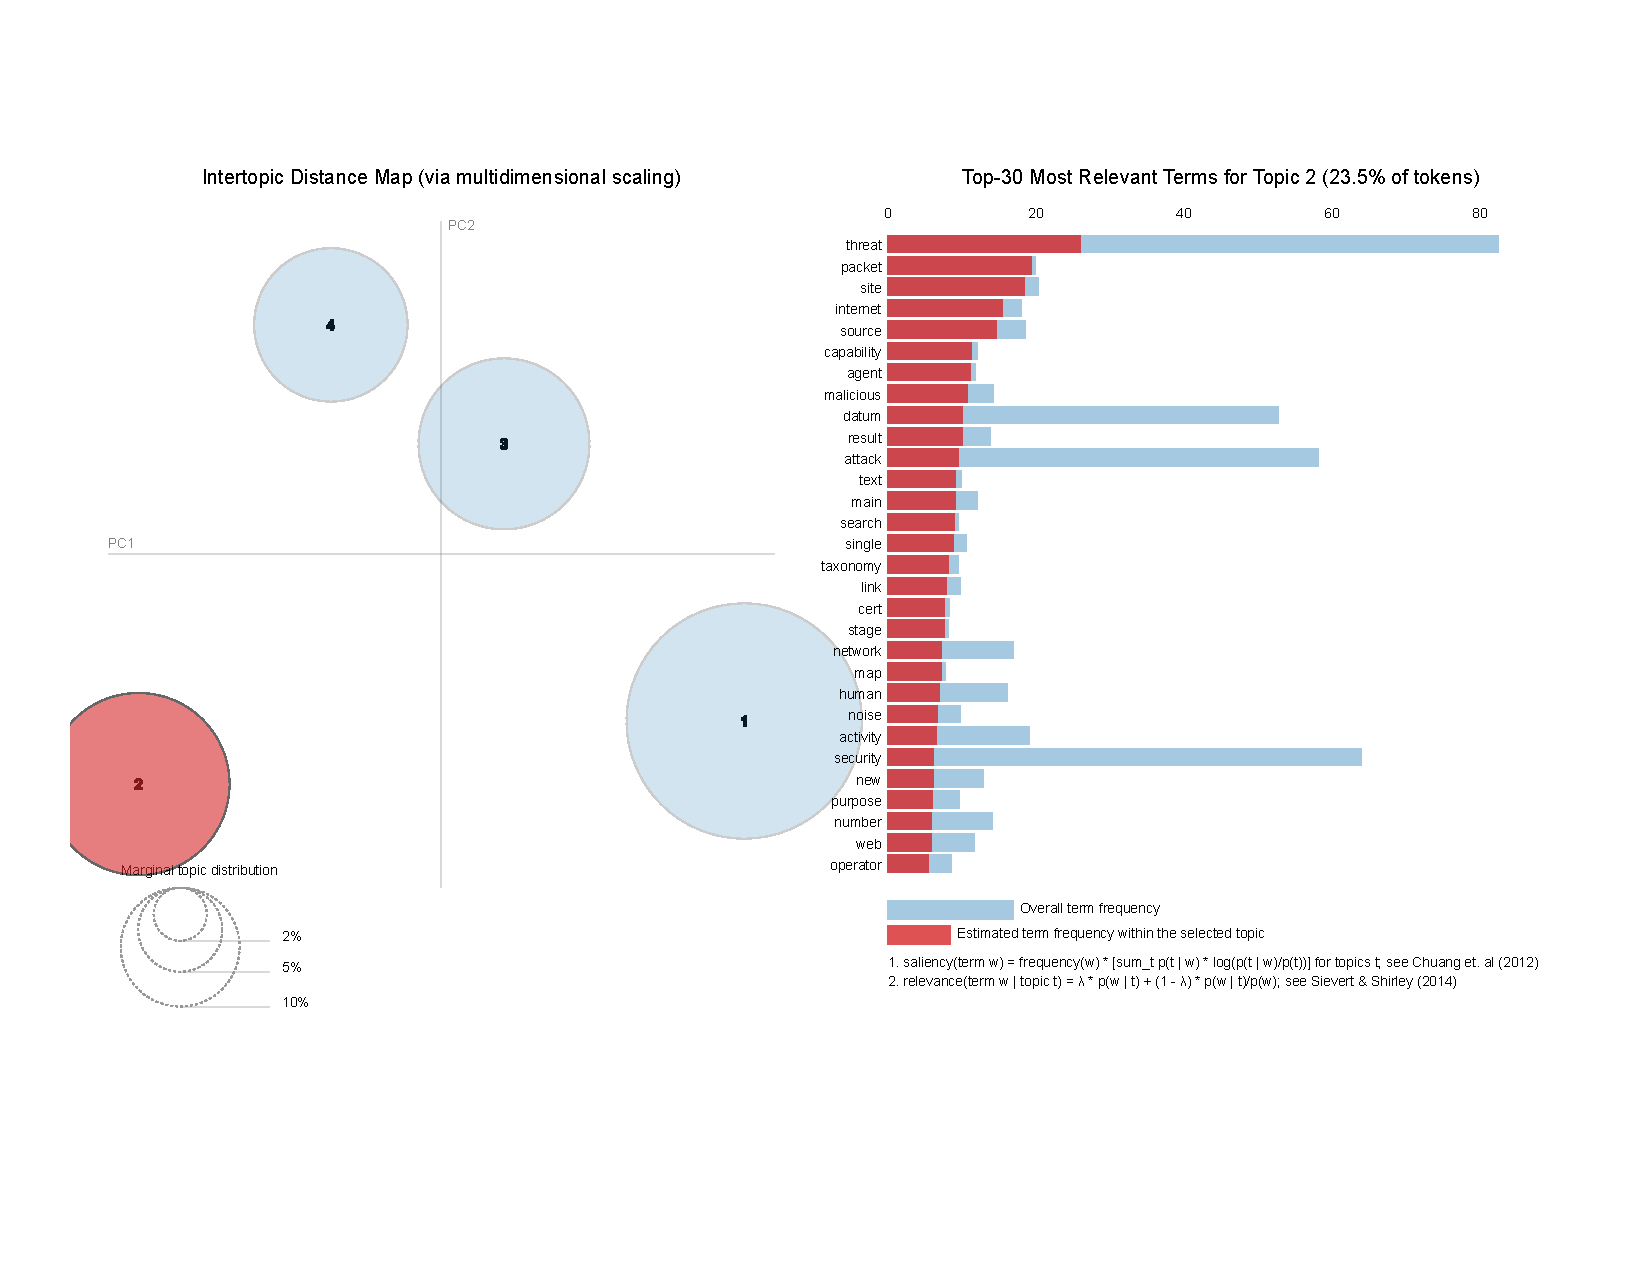
\includegraphics[scale=0.4]{./img/codingALL_topic2.pdf}
\end{center}
\caption{Topic modelling results of the second topic in Surface Web.}
\label{fig:topicmodelling_2}
\end{figure}



%%%%%%%%%%%%%%% %%%%%%%%%%%%%%% 
%%%%%%%%%%%%%%% %%%%%%%%%%%%%%% 
%%%%%%%%%% TABLE topic 3 %%%%%%%%%%%%%%


\begin{table}[h!]
\small
\resizebox{\textwidth}{!}{%
\begin{tabular}{@{}lll@{}}
\toprule
\textbf{Terms} & \textbf{Score} & \textbf{} \\ \midrule 
\rowcolor[HTML]{EFEFEF} 
Process & 7 & \begin{tabular}[c]{@{}l@{}}Processes are all the related activities (parts) inside the system that work together to make it function. \\ A compromised process can lead to a unstable system. In order to compromise a process we have \\ different type of attacks, virus, worm, malware, spyware, trojans. All this attacks have as a target the \\ processes of the system in order to change the main functionalities and make them working for the \\ attacker. In order to avoid this type of attacks is extremely important to have an updated system, a\\ proper antivirus installed and a firewall in order to defend the system environment.\end{tabular} \\
Bitcoin & 4 & \begin{tabular}[c]{@{}l@{}}Bitcoin is either virtual currency or reference to the technology. You can make transactions by check, \\ wiring, or cash. In the last years we witnessed a huge growth of this king of currency and transactions.\\ As a virtual currency, Bitcoins, can also ensure an high level of anonimity and for that reason is widely \\ used for illegal transactions. In the last year we saw bitcoins used for ask ransom after a cyberattack, \\ their extensively use in Dark and Deep web for illegal trafficking and the adoption of this virtual currency\\ in all those activities that need an high level of anonimity.\end{tabular} \\
 &  &  \\
 &  &  \\ \bottomrule
\end{tabular}
}
\caption{Topic analysis results of the third topic for Surface Web.}
\label{tab:topicmodelling_3}
\end{table}


%%%%%%%%%%%%%%% ANALIS TOPIC 3

\begin{figure}
\begin{center}
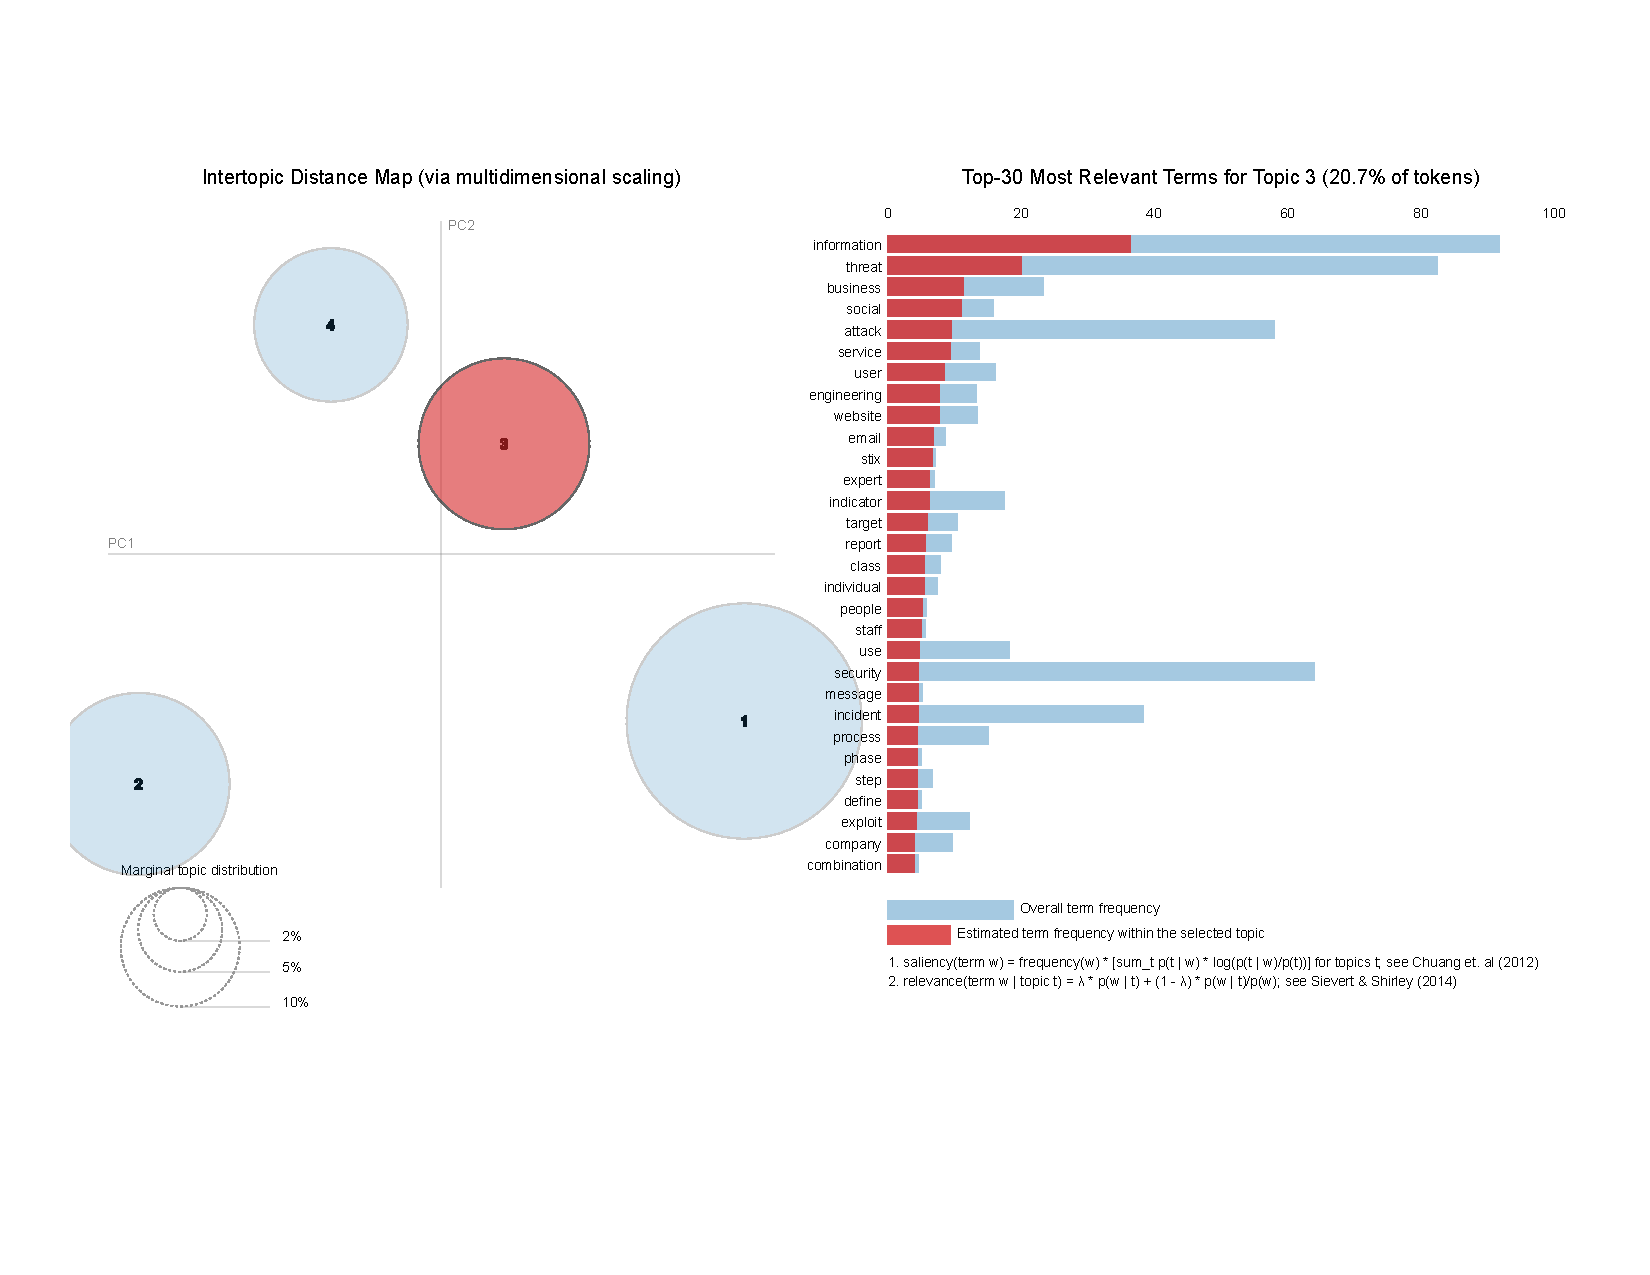
\includegraphics[scale=0.4]{./img/codingALL_topic3.pdf}
\end{center}
\caption{Topic modelling results of the third topic in Surface Web.}
\label{fig:topicmodelling_3}
\end{figure}

%%%%%%%%%%%%%%% %%%%%%%%%%%%%%% 
%%%%%%%%%%%%%%% %%%%%%%%%%%%%%% 
%%%%%%%%%% TABLE topic 4 %%%%%%%%%%%%%%






%%%%%%%%%%%%%%% ANALIS TOPIC 4

\begin{figure}
\begin{center}
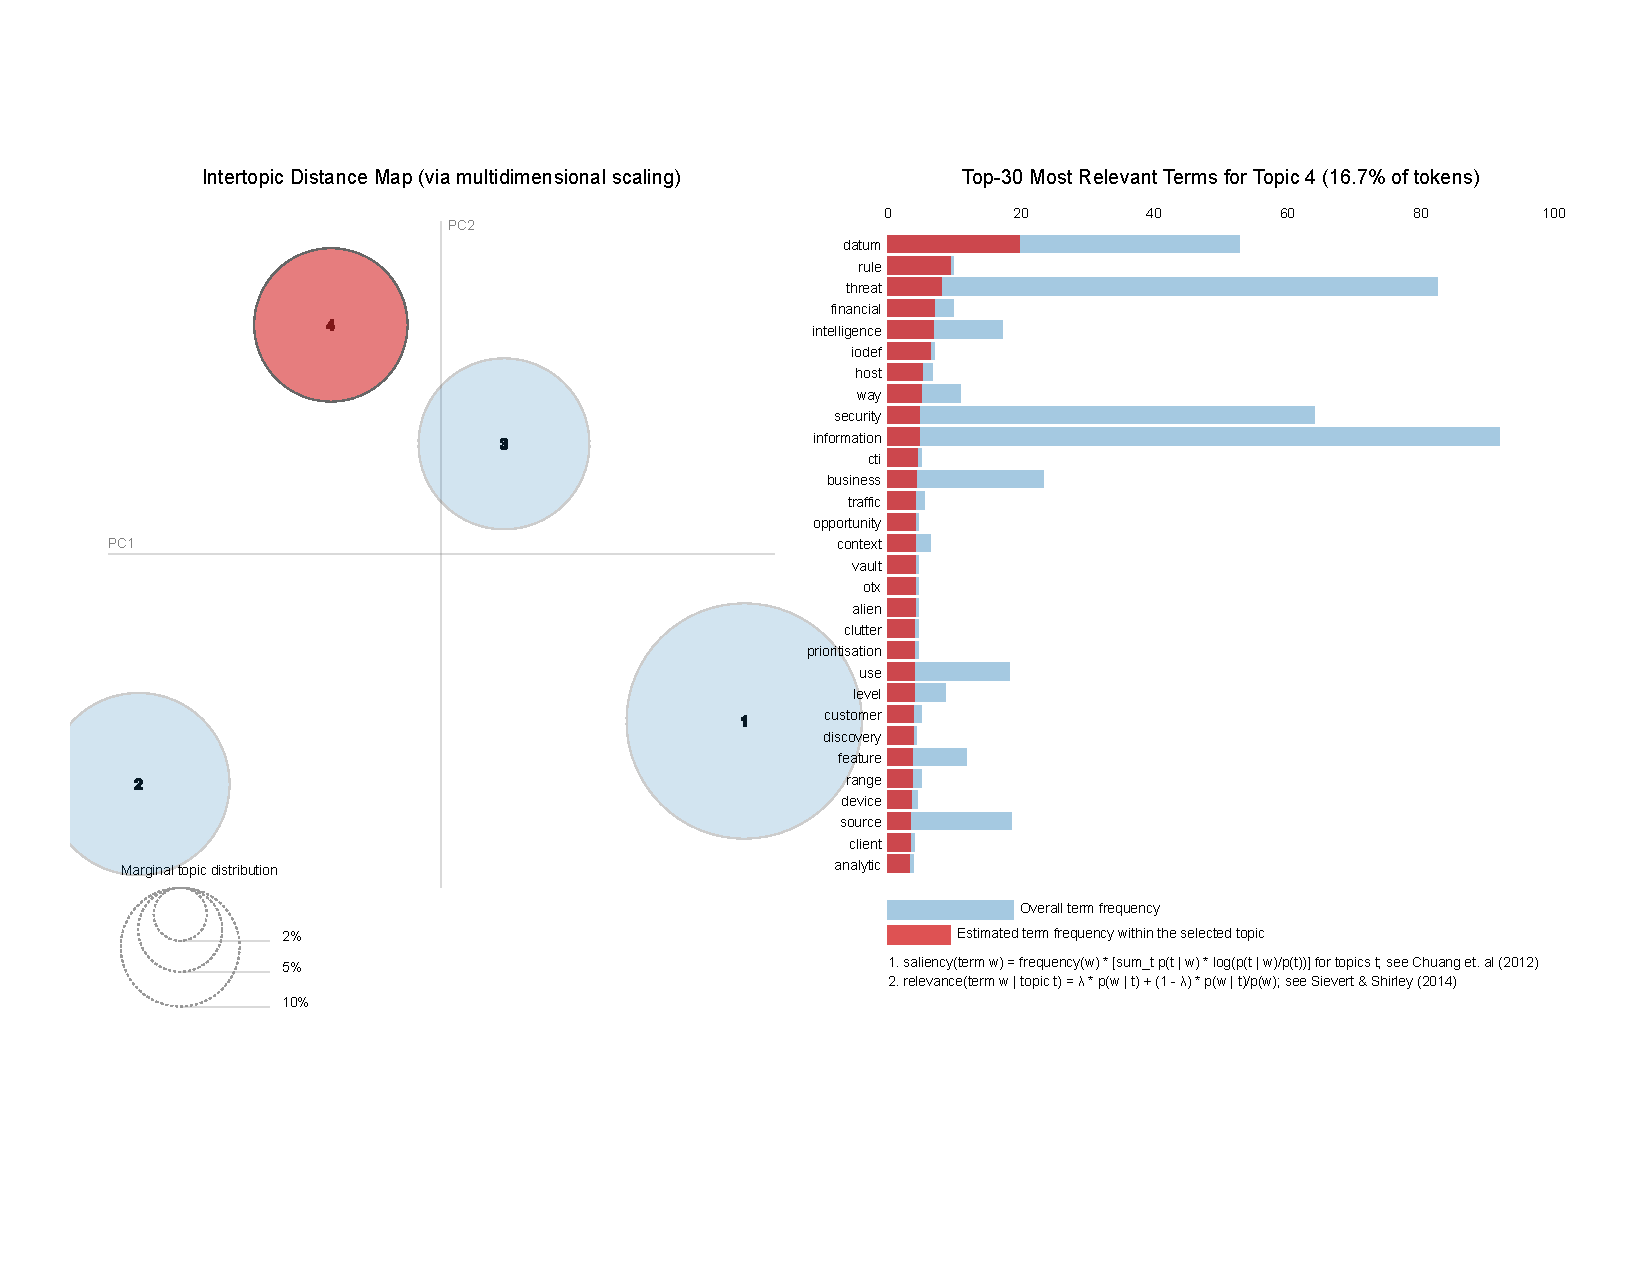
\includegraphics[scale=0.4]{./img/codingALL_topic4.pdf}
\end{center}
\caption{Topic modelling results of the third topic in Surface Web.}
\label{fig:topicmodelling_4}
\end{figure}






\subsubsection{Topic modelling results for Dark and Deep Web}


















